\section{Neural network settings}\label{ap:NNset}
\begin{table}[]
	\centering
	\caption{Parameters of the compared architectures.\label{tab:architectures}}
	\begin{tabular}{|l|l|l|l|l|l|}
		\hline
		& \textbf{compact}                                                  & \textbf{compact classifier}                                       & \textbf{compact classifier dilated}                               & \textbf{\begin{tabular}[c]{@{}l@{}}compact classifier\\  dilated + concat\end{tabular}} & \textbf{\begin{tabular}[c]{@{}l@{}}vgg16 compact \\ + classifier\end{tabular}} \\ \hline \hline
		\multicolumn{6}{|l|}{\textbf{dataset parameters}} \\ \hline
		\textit{Color space}               &   YCbCr and CIELab           &   CIELab        &        CIELab                      &         CIELab                       &     CIELab                                      \\ \hline
		\textit{Fruit dataset}             & Yes                                                               & Yes                                                               & Yes                                                               & Yes                                                                                      & Yes                                                                            \\ \hline
		\textit{Landscape dataset}         & Yes                                                               & No                                                                & No                                                                & No                                                                                       & No                                                                             \\ \hline \hline
		\multicolumn{6}{|l|}{\textbf{Hyperparameter}} \\ \hline 
		\textit{Training method}           & \begin{tabular}[c]{@{}l@{}}ADADELTA\\  with momentum\end{tabular} & \begin{tabular}[c]{@{}l@{}}ADADELTA\\  with momentum\end{tabular} & \begin{tabular}[c]{@{}l@{}}ADADELTA\\  with momentum\end{tabular} & \begin{tabular}[c]{@{}l@{}}ADADELTA with \\ momentum\end{tabular}                        & \begin{tabular}[c]{@{}l@{}}ADADELTA\\  with momentum\end{tabular}              \\ \hline
		\textit{Epochs trained}            &     50       &     28  &     30   &     30                                                                                     &      25                                                                          \\ \hline
		\textit{Batch size}                &         20                                                          &     20                                                              &       20                                                            &        20                                                                                  &   20                                                                            \\ \hline \hline
		\multicolumn{6}{|l|}{\textbf{Architecture properties}} \\ \hline 
		\textit{Front end module}          & trained from scratch                                              & trained from scratch                                              & trained from scratch                                              & trained from scratch                                                                     & VGG16 front end                                                                \\ \hline
		\textit{Max pool}                  & Yes                                                               & Yes                                                               & No                                                                & No                                                                                       & Yes                                                                            \\ \hline
		\textit{Strides}                   & No                                                                & No                                                                & Yes                                                               & Yes                                                                                      & No                                                                             \\ \hline
		\textit{dilation}                  & No                                                                & No                                                                & Yes                                                               & Yes                                                                                      & No                                                                             \\ \hline
		\textit{Concatenation}             & Yes                                                               & Yes                                                               & No                                                                & Yes                                                                                      & Yes                                                                            \\ \hline
		\textit{Kernel size}               & 3x3                                                               & 3x3                                                               & 3x3                                                               & 3x3                                                                                      & 3x3                                                                            \\ \hline
		\textit{Activation function}       & ReLu                                                              & ReLu                                                              & ReLu                                                              & ReLu                                                                                     & ReLu                                                                           \\ \hline
		\textit{Batch norm}                & Yes                                                               & Yes                                                               & Yes                                                               & Yes                                                                                      & Yes                                                                            \\ \hline \hline
		\multicolumn{6}{|l|}{\textbf{Classification properties}} \\ \hline  
		\textit{Annealed mean temperature} &                                                                   &                                                                   &                                                                   &                                                                                          &                                                                                \\ \hline
		\textit{K-nearest neighbour}       & -                                                                 & 10                                                                & 10                                                                & 10                                                                                       & 10                                                                             \\ \hline
		\textit{K-nearest neighbour sigma} & -                                                                 & 5                                                                 & 5                                                                 & 5                                                                                        & 5                                                                              \\ \hline
		\textit{Number of colorbins} & -                                                                 & 247                                                                 & 247                                                                 & 247                                                                                        & 247                                                                              \\ \hline
	\end{tabular}
\end{table}


\section{More results}\label{ap:more_results}
\begin{figure}[h]
	\centering
	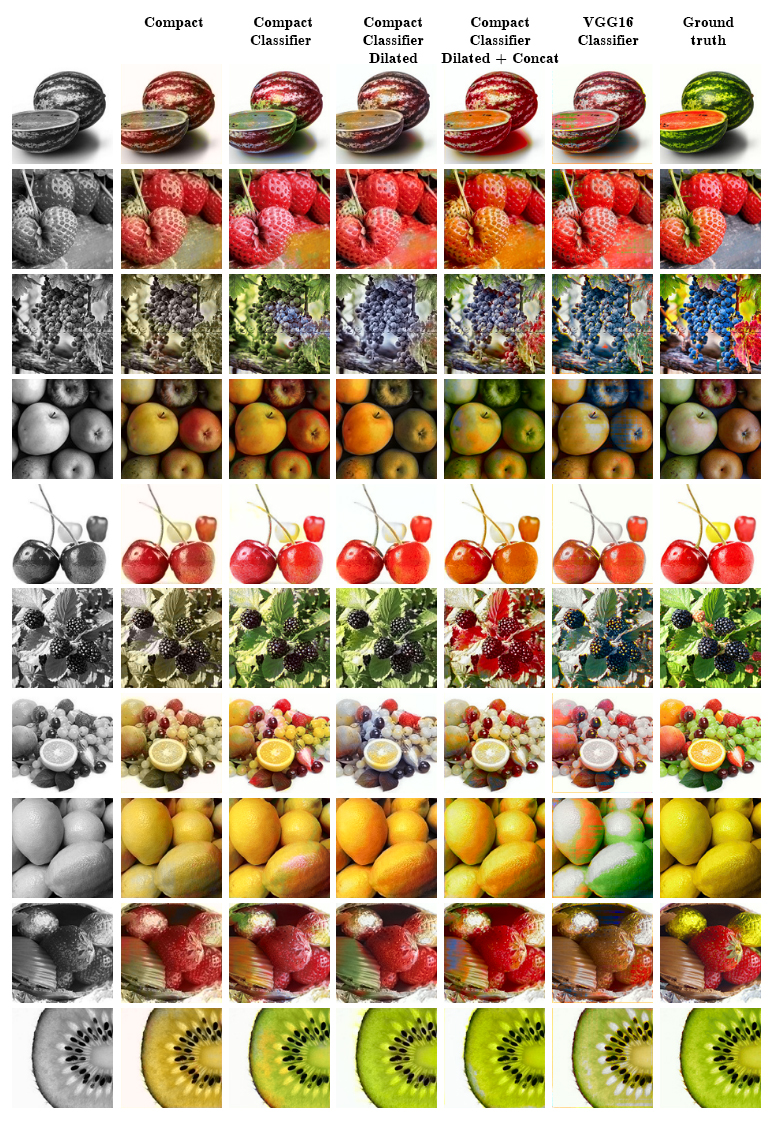
\includegraphics[width=0.9\textwidth]{set1}
\end{figure}


